\chapter{Week 5: 16\textsuperscript{th} - 22\textsuperscript{nd} February }

\begin{itemize*}
	\item Interface with GPS module 
	\item  Test the control and filter code on the quad-rotor
	\item Use the Kalman Filter to filter the GPS
\end{itemize*}

 \tocless\section{Testing }
Most of the week was sent testing the control and filters on the quad-rotor. It was found that the delay on the second order complementary filter was to large so the Kalman filter was implemented on the chip. The first order filter was also investigated to see if the delay could be reduced, it was and the results of the filtering can be seen in figure \ref{Fig: Kalman Filter Estimate and First Order complementary Filter}:-



						\begin{figure}[h]
							\centering
							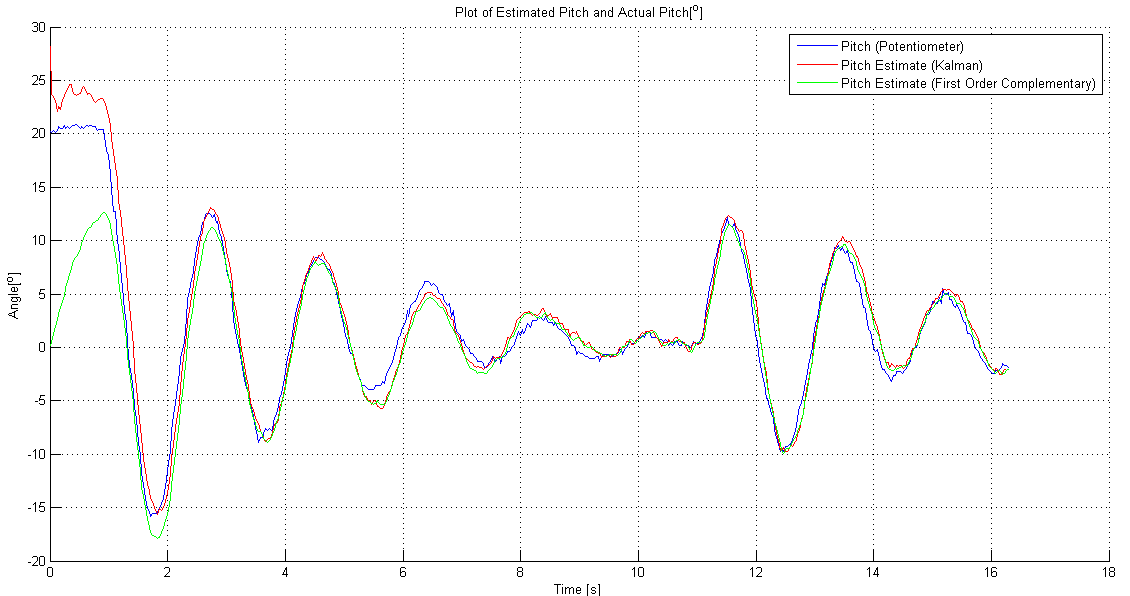
\includegraphics[width =0.7\paperwidth, height = 10cm]{\DocRoot/images/First_order_filter_vs_kalman}
							\caption{Plot of Kalman Filter Estimate, First Order complementary Filter and Actual Angle of the device}
							\label{Fig: Kalman Filter Estimate and First Order complementary Filter}
						\end{figure}
						
Note as the findings in figure \ref{Fig: Kalman Filter Estimate and First Order complementary Filter} are promising the filter overshoots when there is high accelerations, the Kalman Filter doesn't have such draw backs. The complementary filter presented in figure \ref{Fig: Kalman Filter Estimate and First Order complementary Filter} has a filter parameter of $\tau = 0.5$.						


 \tocless\section{GPS Mapping \& Associated Equations}	

If one wants to control the quad-rotor using differential equations based on $x,y,z$ coordinate system one will have to map the latitude (\gls{latitude}) and longitude (\gls{longitude}) values given by the \gls{gps} sensor.	Note that any mapping \enquote{unwrapping} of a spherical objecting onto a flat plane will cause distortions and loss of information (this was first mathematically proven by C. F. Gauss). Methods of doing this mapping will now be presented:-

 \tocless\subsection{Transverse Mercator Projection}
 The Transverse Mercator Projection or Gauss–Kr\"{u}ger projection is a conformal mapping of the earth ellipsoid where a central meridian is mapped into a straight line at constant scale. It is widely used in national and international mapping systems around the world and hits a middle ground between computational ease and accuracy. In order to preform this projection one places a model of the Earth on a cylinder as seen in figure \ref{Fig:  Transverse_Mercator_projection} and \enquote{roll} the cylinder to form a conventional map\cite{utm}.
 
 
 \begin{figure}[h]
 	\centering
 	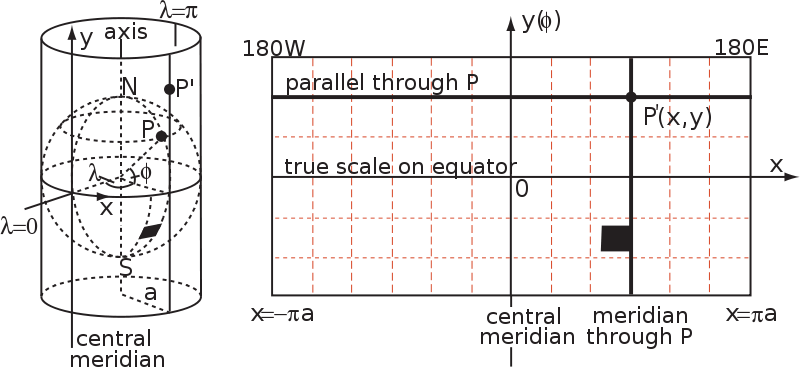
\includegraphics[width =0.7\paperwidth]{\DocRoot/images/Transverse_Mercator_projection}
 	\caption{Normal aspect of a tangent cylindrical project of a sphere (Transverse Mercator projection)}
 	\label{Fig:  Transverse_Mercator_projection}
 \end{figure}
 
 Using the project defined by figure \ref{Fig:  Transverse_Mercator_projection} one can calculate \gls{east} \& \gls{north} coordinates using the following assuming the $y$-axis goes through the  Prime Meridian in Greenwich. 
 \begin{align}
\begin{split}
 \gls{east}(\gls{longitude},\gls{latitude}) &= \frac{1}{2}k_o a \ln\left[\frac{1 + \sin\gls{longitude}\cos\gls{latitude}}{1 - \sin\gls{longitude}\cos\gls{latitude}}\right]\\
 \gls{north}(\gls{longitude},\gls{latitude}) &= k_o a \arctan\left[\sec\gls{longitude}\cos\gls{latitude}\right]
\end{split}
 \end{align}
 
 Similarity, if one can to find latitude and longitude using  only \gls{east} \& \gls{north} one can use the following equations:-
 
  \begin{align}
  \begin{split}
  \gls{longitude} &= \arctan\left[\sinh\frac{\gls{east}}{k_oa} \sec\frac{\gls{north}}{k_oa}\right]\\
  \gls{latitude}(\gls{east},\gls{north}) &= k_o a \arctan\arcsin\left[\mathrm{sech}\frac{\gls{east}}{k_oa}\sin\frac{\gls{north}}{k_oa}\right]
  \end{split}
  \end{align}
  
  where:-\\
  $k_o$; is the \enquote{point scale}  and is commonly taken as  0.9996 for reasons that will not be mentioned here but are listed in \cite{utm}\\
  $a$; is the equatorial radius of the earth and is equal to 6,378,137~$m$\\
  $b$; is the polar radius of the earth and is equal to 6,356,752.3142~$m$
  
   \tocless\subsection{Universal Transverse Mercator}
 The \gls{utm} projection uses a 2-D Cartesian based system to map the locations on the surface of the earth. Note this system differs from the traditional method of latitude (\gls{latitude}) and longitude (\gls{longitude}) as it is not a single map projection.  \gls{utm} also divides the Earth into sixty \enquote{Zones} , which are six-degree bands of longitude (\gls{longitude}) and it uses the Transverse Mercator Projection in each of these \enquote{Zones} \cite{utm}.
 
 The following formulas are truncated version of the Transverse Mercator: flattening series, these formulae where first derived by J.H.L Kr\"{u}ger in 1912. The mapping use WGS 84 which describes the Earth as an oblate spheroid. In order to map from latitude and longitude (\gls{latitude},\gls{longitude}) to \gls{utm} (\gls{east},\gls{north}) one has to introduce constants to make the notation easier, this is done first:-
 
 \begin{align}
 \begin{split}
 n                 &= \frac{f}{2-f},~~                                                                                           A=\frac{a}{1+n}\left(1 + \frac{1}{4}n^2 + \frac{1}{64}n^4 + \dddot{}\right)\\
 \alpha_1 &= \frac{1}{2}n - \frac{2}{3}n^2 + \frac{5}{16n^3} + \dddot{},       ~~\alpha_2 = \frac{13}{48}n^2 - \frac{3}{5}n^3 + \dddot{},     ~~\alpha_3   = \frac{61}{240}n^3 + \dddot{}\\
 \beta_1    &= \frac{1}{2}n - \frac{2}{3}n^2+\frac{37}{96}n^3 + \dddot{},      ~~\beta_2   = \frac{1}{48}+\frac{1}{48}n^3 + \dddot{},              ~~  \beta_3   = \frac{17}{480}n^3 + \dddot{}\\
 \delta_1  &=  2n-\frac{2}{3}n^2 - 2n^3 + \dddot{},                                                      ~~ \delta_2 = \frac{7}{3}n^2 - \frac{8}{5}n^3 + \dddot{},          ~~   \delta_3 =   \frac{56}{15}n^3  + \dddot{} 
 \end{split}
 \end{align}
 
 Where: \\
 $f$: is flatting and is given by the following:- $f = (a-b)/a$ \\
 $e$: is the eccentricity of the earth and is defined as follows:- $e= \sqrt{f(2-f) }$\\


 \tocless\subsubsection{Mapping from latitude and longitude (\gls{latitude},\gls{longitude}) to \gls{utm} (\gls{east},\gls{north})}
Before one can project (\gls{latitude},\gls{longitude}) to \gls{utm} (\gls{east},\gls{north}) one has to do an interment step\footnote{Please see the following for more details and a full derivation of these formulas \cite{utm}}.

\begin{align}
	\tau^\prime &= \sinh \left(\tanh^{-1}(\sin\gls{latitude})- \frac{2\sqrt{n}}{1+n}\tanh^{-1}\left(\frac{2\sqrt{n}}{1+n}\sin\gls{latitude}\right) \right)\\
	\xi^\prime &= \tan^{-1}(\frac{\tau^\prime}{\cos(\gls{longitude} - \lambda_o)})\\
	\eta^\prime &= \sinh^{-1}\left(\frac{\sin(\gls{longitude}-\lambda_o)}{\sqrt{\tau^{\prime 2} + \cos^2\gls{longitude}}}\right)
\end{align}
	
Now that these are defined one can map 	 (\gls{latitude},\gls{longitude}) to \gls{utm} (\gls{east},\gls{north})  using the following formulas:-	

\begin{align}
\gls{east} =& k_oA\left(	\eta^\prime  + \sum_{j=1}^{3}\alpha_j\cos(2j\xi^\prime)\sinh(2j\eta^\prime)\right)\\
\gls{north} =& k_oA\left(	\xi^\prime  + \sum_{j=1}^{3}\alpha_j\sin(2j\xi^\prime)\cosh(2j\eta^\prime)\right)
\end{align}

   \tocless\subsection{Basic Method of Mapping  (\gls{latitude},\gls{longitude}) to (\gls{east},\gls{north})}
  For small angles ($1^o$) one can use the following equations:-
  
  \begin{equation}
  \Delta_{\gls{latitude}} = \frac{\pi a (1 - e^2)}{180(1-e^2\sin^2\gls{latitude})^{\frac{3}{2}}} \label{eq: delta latitude}
  \end{equation}
 
 The distance in meters (correct to 0.01 metres) between ($\gls{latitude} \pm 0.5^o$) on the \gls{wgs} 84 spheroid is given by the following formula:-
 
 \begin{equation}
  \Delta_{\gls{latitude}} =  111132.954 - 559.822\cos(2\gls{latitude}) + 1.175\cos(4\gls{latitude})
 \end{equation}
 
 Similarly  for longitude:-
   \begin{equation}
   \Delta_{\gls{longitude}} = \frac{\pi a \cos(\gls{latitude})}{180\sqrt{1-e^2\sin^2\gls{latitude}}} \label{eq: delta longtitude}
   \end{equation}
